\chapter{Analyse en ontwerp}
Uit de probleemstelling werd het snel duidelijk dat het probleem omtrent het Python testraamwerk complexer is dan op het eerste zicht lijkt.
In dit hoofdstuk zal het probleem verder geanalyseerd worden.
Aan de hand van deze bevindingen gaat een architectuur en structuur ontworpen worden.
Deze vormen de basis voor de implementatie van de demo.

\section{Analyse}
%Packager
Een probleemanalyse onthulde al snel dat dit probleem onder te verdelen is in verschillende deelproblemen.
Het framework bestaat uit verschillende componenten, hieronder vallen de drivers en bibliotheken.
Elke component heeft een unieke installatiewijze en de componenten moeten in een specifieke volgorde geïnstalleerd worden.
Hiernaast moeten verscheidene componenten geconfigureerd worden aan de hand van een configuratiebestand.
Dit configuratiebestand is doelsysteem specifiek.
Tijdens het onderzoek zal er onderzocht welke technologieën gebruikt zal worden om al deze componenten te combineren tot één uitvoerbaar bestand.
Bij het selectieproces moet er rekening gehouden worden met de toekomst.
Er wordt best een technologie gekozen die cross-platform is, zodanig dat het bedrijf niet beperkt wordt in de toekomst.

%Server
De probleemanalyse onthulde ook dat de verschillende executables verspreidt moeten worden.
Door dit proces te automatiseren, is het mogelijk om waardevolle informatie te verzamelen.
Hiermee zouden rapporten gegeneerd kunnen worden voor het bedrijf.
Tijdens het ontwerpen zal schaalbaarheid een belangrijke factor spelen.
Naar de toekomst toe zal het aantal systemen waarop de applicatie geïnstalleerd wordt toenemen.

%Environment
Zoals reeds hierboven vermeld, is het installatieproces foutgevoelig.
Na de foutanalyse bleek dat hiervoor een schaalbare oplossing voor gevonden moet worden.
Bij het finaliseren van een component installatie, moeten de functionaliteiten van de component gecontroleerd worden.
Mocht deze incorrect functioneren dan moet een gepaste actie, eventueel een rollback, gebeuren. 
Ook na de volledige installatie moet gecontroleerd worden of het geheel correct functioneert.
Hierdoor wordt er voorkomen dat er nodeloos veel tijd verloren gaat in het herinstalleren van de applicatie.
Robuustheid zal een belangrijke component zijn tijdens de ontwerpfase.
Bij het ontwerpen moet gebruiksvriendelijkheid in het achterhoofd gehouden worden.

Na de probleemanalyse werd het al snel duidelijk dat het werk op te delen valt in drie grote componenten.
Deze drie onderdelen zullen de basis vormen voor de architectuur en zullen gebruikt worden als leidraad.
Het eerste onderdeel zal bestaan uit een packager met als doel het inpakken van de nodige drivers, bibliotheken, ... .
Naast de packager is er een deployment server nodig die instaat voor het verspreiden van de installers die de packager aflevert.
Dankzij het automatiseren van de deployment, kan het installatieproces per client getrackt worden. %getrackt is juist
Om deze stap te vereenvoudigen, moet aan de client-side een deployment environment voorzien worden.
In die omgeving wordt de installatie geïsoleerd.
Mocht een rollback nodig zijn, dan kan deze op een eenvoudige manier gebeuren.

Gedurende deze thesis wordt een prototype ontworpen.
In Figuur~\vref{fig:overzichtsDiagram} wordt de algemene structuur van de applicatie weergegeven.
Met behulp van deze basis is het mogelijk om een demo te produceren die de verschillende problemen verhelpt.

\begin{figure}[!hbt]
\centering
  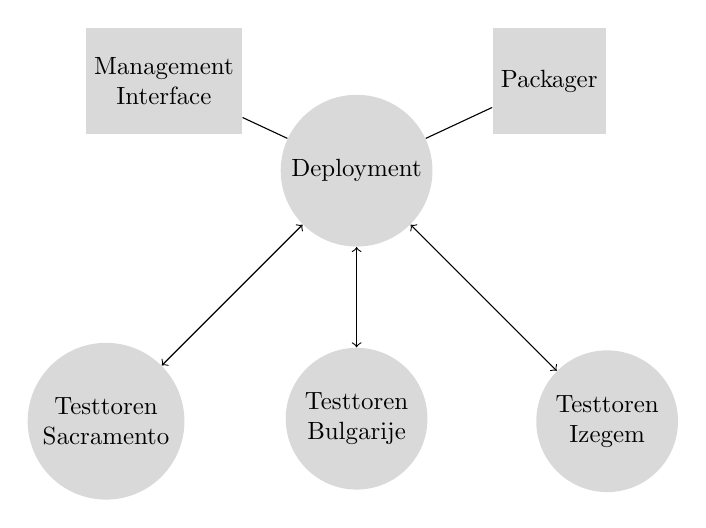
\begin{tikzpicture}[scale=.9, transform shape]
\tikzstyle{every node} = [circle, minimum size = 2cm, fill=gray!30]
\node (a) at (0, 0) {Deployment};
\node[shape = rectangle,minimum size = 1.5cm] (packager) at +(25: 3) {Packager};
\node[shape = rectangle,minimum size = 1.5cm, align=center] (logger) at +(155: 3) {Management\\ Interface};
\node[align=center] (b) at +(225: 5) {Testtoren\\ Sacramento};
\node[align=center] (c) at +(270: 3.5) {Testtoren\\ Bulgarije};
\node[align=center] (d) at +(315: 5) {Testtoren\\ Izegem};
\foreach \from/\to in {a/b, a/c, a/d}
\draw [<->] (\from) -- (\to);
\draw [-] (a) -- (packager);
\draw [-] (a) -- (logger);
\end{tikzpicture}
  \caption{Overzichtsdiagram van de algemene structuur}
  \label{fig:overzichtsDiagram}
\end{figure}

\section{Databank}\label{sec:databank}
Het aantal pakketten die gebruikt gaan worden, gaan alleen toenemen.
Naast deze groei zullen ook het aantal gebruikers toenemen.
Daarom werd er geopteerd om een databank te ontwerpen voor het opslaan van alle cruciale data.
In overleg met het bedrijf werd ervoor gekozen om MySQL te gebruiken als managementsysteem.
Het ontwerp van de databank is terug te vinden in Figuur~\vref{fig:databank}.

\begin{figure}[!ht]
\centering
\makebox[0pt]{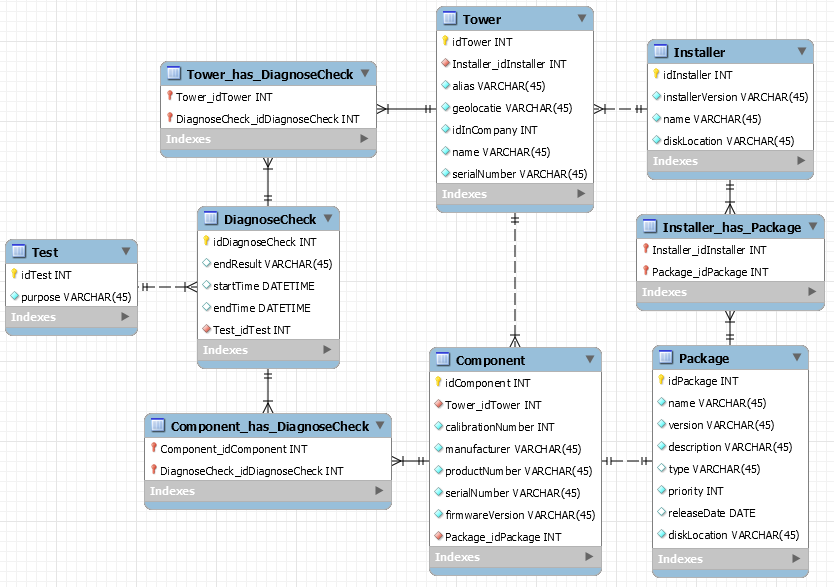
\includegraphics[scale=0.7]{afbeelding/databankOntwerp.png}}
\caption{Ontwerp van de databank}
\label{fig:databank}
\end{figure}

Tijdens het ontwerp van de databank, in overleg met het bedrijf, zijn er verschillende keuzes gemaakt die moeten toegelicht worden.
Dit ontwerp weerspiegelt de structuur die aangehaald werd in Figuur~\vref{fig:overzichtsDiagram} met als verschil dat in het ontwerp de client centraal staat en niet de server.
Verder zullen de verschillende tabellen overlopen worden en enkele termen vastgelegd worden zodanig dat deze een eenduidige betekenis gedurende de rest van de thesis.
Centraal staan alle tabellen horende bij de een testtoren.
Iedere toren heeft een ID, naam en serienummer. 
De combinatie van deze drie waarden zijn uniek binnen het bedrijf.
Aangezien deze combinatie niet betekenisvol is, wordt er een alias gekoppeld aan iedere toren.
Elke toren bevat verschillende hardware componenten, zoals voedingen of netwerkkaarten, die nodig zijn om testen uit te voeren.
Iedere component is gemaakt door een bepaalde fabrikant en krijgt daar een serienummer.
Vanuit het bedrijf wordt er nummer toegekend aan iedere component die gebruikt wordt om de calibratie te achterhalen.
Naast het calibratienummer heeft een component een firmware versie.

Rechts van de client bevinden zich alle tabellen die horen bij de packager.
De packager levert verschillende installers af die bestaan uit packages.
Iedere package heeft een naam en versienummer die uniek is.
Bij iedere package wordt bijgehouden welk type package het is, de prioriteit voor de installatievolgorde, een korte beschrijving en de release datum.
Een package wordt gekoppeld aan een installer maar kan gebruikt worden in verschillende installers.
Uiteraard draait op iedere toren een bepaalde installer en wordt één installer gebruikt op verschillende torens.

Aan de linkerzijde bevinden zich de tabellen die horen bij het logger gedeelte.
Tijdens het installeren van het framework kunnen verschillende tests uitgevoerd worden om te testen of een component correct is geïnstalleerd.
Op basis van de gegevens van een component kan, bij het falen van de test, gecontroleerd worden wat bijvoorbeeld de firmware versie van de component is.
Ook na de volledige installatie van het framework kan een test uitgevoerd worden zodat gecontroleerd wordt of de connecties tussen de componenten goed werkt.

\subsection{Architectuur}

\subsubsection{Packager}
De architectuur van de packager wordt gebaseerd op de architectuur en structuur van het Qt installer framework.
Hierbij wordt bedoelt dat één overkoepelende installer wordt geproduceerd die bestaat uit verschillende kleine componenten.
Het Qt installer framework wordt hiervoor niet zelf gebruikt.
Deze keuze werd gemaakt op basis van verschillende argumenten.
%het zorgt voor een beter bereik van de verschillende packages -> kunnen test tussendoor uitvoeren
Door het personaliseren van de packager, is het mogelijk om iedere stap in het deployment proces te personaliseren.
Op deze manier kan na het installeren van een pakket een verbeterde afhandeling plaats vinden.
Een test kan uitgevoerd worden op het einde van de installatie, een handeling die met het Qt installer framework mogelijk is maar moeilijk te realiseren is.
%geen gedoe met docker
Doordat een gepersonaliseerde packager wordt ontworpen, worden problemen met Docker vermeden.
In de deployment environment wordt Docker gebruikt om verscheidene problemen met het deployment proces op te vangen (dit wordt verder besproken).
De Docker omgeving, zoals reeds vermeld in Sectie~\vref{sec:virtualisatie}, gebruikt van LXC.
Het besturingssysteem van de containers aan de client side is hierdoor Linux.
Windows gebruiken als besturingssysteem is mogelijk maar deze optie staat nog altijd in beta schoenen.
De installer geproduceerd door het Qt installer framework moet dus compatibel zijn met Linux.
Dit is mogelijk met het framework maar de productie van de installer moet ook plaatsvinden in een Linux besturingssysteem.
Om dit te realiseren zou Docker gebruikt kunnen worden zodanig dat er een abstractie gedaan wordt van het host besturingssysteem.
Zo'n opstelling creëren, waarbij een container gebruikt wordt met het Qt installer framework in verwerkt, brengt meer werkt en is omslachtiger ten opzichte van het zelf fabriceren van een packager met een gelijkaardige structuur en gelijkaardige functionaliteiten.

%%% TODO schrijven hoe het er dan wel uit gaat zien
De packager gaat een gelijkaardige structuur hebben als het Qt installer framework.
Om de packager te maken wordt Python gebruikt als programmeertaal.
Een installer bestaat uit verschillende pakketten en functioneert als overkoepelend geheel.
Per test framework wordt één installer geassocieerd.
Voor alle drivers/bibliotheken die nodig zijn, worden verschillende pakketten voorzien waarbij één driver hoort bij één pakket.
Ieder pakket bestaat uit twee delen: een data en metadata gedeelte.
Het data gedeelte bevat de effectieve driver/bibliotheek en het metadata gedeelte bevat de nodige beschrijving van het pakket in de vorm van een ``package.json''.
Hiernaast zijn verschillende scripts aanwezig die gebruikt worden voor een gepersonaliseerde installatie.
De structuur van een mogelijke installer is terug te vinden in Figuur~\vref{fig:installerStructuur}.
In het voorbeeld wordt een installer opgebouwd bestaande uit twee delen.
Het eerste deel bestaat uitsluitend uit configuratie bestanden en het tweede deel bestaat uit de pakketten.
De twee onderdelen zijn terug te vinden in de rode rechthoek.
Verder worden de packages ook opgedeeld in twee categorieën.
De eerste categorie is cruciaal voor de correcte werking van het test framework.
Dit onderdeel bestaat uit een versie van het test framework gecombineerd met de pakketten die nodig zijn voor een fatsoenlijke werking (deze pakketten worden aangegeven door de gele rechthoek).
Hiernaast is er één pakket aanwezig die niet cruciaal is voor het testraamwerk maar wel nodig is om een correcte werking te verzekeren op de site zelf (aangegeven door de groene rechthoek).
Deze bevindt zich in de tweede categorie.

\begin{figure}[!ht]
\centering
\makebox[0pt]{\includegraphics[scale=0.5]{afbeelding/installerStructuur.png}}
\caption{Structuur van een installer bestaande uit drie pakketten}
\label{fig:installerStructuur}
\end{figure}

Om een dergelijke structuur op te bouwen, werkt de packager nauw samen met de databank waarin alle informatie vervat zit.
Het ontwerp van de databank werd al uitvoerig besproken in Sectie~\ref{sec:databank} en is terug te vinden in Figuur~\ref{fig:databank}.

\subsubsection{Deployment server}
Het centrale systeem in de architectuur is de deployment server.
Zoals reeds uitgelegd zal dit onderdeel instaan voor het verspreiden van de verschillende installers en functioneren als een verzamelcenter voor alle informatie.
De architectuur van de deployment server wordt gebaseerd op de software dock architectuur die besproken werd in Sectie~\vref{sec:softwareDock} en is terug te vinden in Figuur~\vref{fig:softwareDockAangepast}.

\begin{figure}[!ht]
\centering
\makebox[0pt]{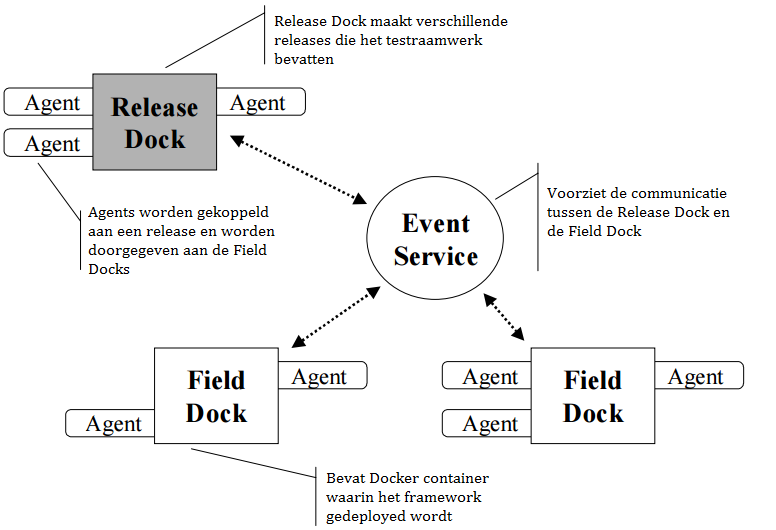
\includegraphics[scale=0.5]{afbeelding/softwareDockAangepast.png}}
\caption{Software Dock Architectuur \citep{hall1999cooperative}}
\label{fig:softwareDockAangepast}
\end{figure}

De software dock architectuur bestaat uit 4 grote componenten, namelijk het release dock, field dock, event service en de agenten.
Het release dock bevindt zich aan de serverzijde en bevat alle software van de packager.
Met hulp van de packager worden verschillende releases geproduceerd.
Als een release klaar is voor deployement wordt een event afgevuurd naar de event service.
Alle agenten die geabonneerd zijn op het gepaste event worden vervolgens op de hoogte gebracht.
Deze gedistribueerde architectuur laat een eenvoudige uitbreiding van het aantal docks toe.
Het tweede type dock dat aanwezig is in de architectuur is de field dock.
De verschillende clients functioneren als een field dock en zullen communiceren met het release dock aan de hand van de event-service.

%%schrijven over hoe de agenten werken en hoe ze gaan werken volgens de handelingen van ORYA
Naast de docks bevat de architectuur agenten.
Deze staan in voor het uitvoeren van allerlei deployment gerelateerde handelingen.
Iedere agent is gekoppeld aan één stap uit de software levenscyclus die besproken werd in Sectie~\vref{sec:softwareLevenscyclus}.
Hiernaast zal aan iedere release van het release dock een subset van alle agenten toegevoegd en verscheept worden naar het field dock.
Zo wordt bijvoorbeeld een agent voorzien die instaat voor het installatieproces.
De agent wordt samen met de release verscheept naar het field dock waarna de agent in actie schiet.
De agent begint met het creëren van een nieuwe Docker container waarin de installer losgelaten kan worden.
Vervolgens zal de agent de installatie aanvangen en zullen de scripts horende bij de pakketten uitgevoerd worden in de container.
Ieder agent zal een bepaalde set van handelingen uitvoeren die overeenkomt met een deployment proces die besproken werd in de ORYA case studie in Sectie~\vref{sec:ORYA}.
Net zoals bij ORYA wordt ieder deployment proces beschreven aan de hand van andere deployment processen en basis activiteiten.
Het creëren van een nieuwe container in de installatie agent wordt gezien als zo'n basis activiteit.
In Figuur~\vref{fig:fieldDock} wordt de algemene structuur van een field dock weergegeven.

\begin{figure}[!ht]
\centering
\makebox[0pt]{\includegraphics[scale=0.5]{afbeelding/fieldDock.png}}
\caption{Structuur van een field dock}
\label{fig:fieldDock}
\end{figure}

Door agenten te gebruiken, een strategie die ook gezien werd in de Atlas case studie in Sectie~\vref{sec:ATLAS}, wordt het mogelijk om alle stappen in de software levenscyclus uniek te behandelen.
Hiernaast kan bij iedere release een andere set van agenten geassocieerd worden waardoor iedere release verder kan gepersonaliseerd worden.
De volledige architectuur is terug te vinden in Figuur~\vref{fig:architectuur}.
In de figuur zijn zowel de packager als de deployment environment toegevoegd.

\begin{figure}[!ht]
\centering
\makebox[0pt]{\includegraphics[scale=0.5]{afbeelding/architectuur.png}}
\caption{Architectuur van het prototype}
\label{fig:architectuur}
\end{figure}

\subsubsection{Deployment environment}
De deployment environment komt overeen met de field dock in de software dock architectuur.
In de omgeving gaat de installer, afkomstig van de packager, uitgevoerd worden zodanig dat het test framework geïnstalleerd wordt.
Aan dit proces zijn de verschillende problemen verbonden die besproken zijn in Sectie~\vref{sec:softwareLevenscyclus}.
Om de verschillende deployment problemen te vermijden en om ervoor te zorgen dat geen uitgebreide rollback strategieën nodig zijn, wordt een geïsoleerde omgeving voorzien waarin de software gedeployed kan worden. 
Dit wordt gerealiseerd aan de hand van virtualisatie technieken, meer bepaald aan de hand van Docker.
Docker wordt verkozen boven een gewone virtuele machine omdat het uitvoeren van handelingen (zoals opstarten, stoppen, \ldots) op een container minder resources en tijd vraagt in vergelijking met een virtuele machine.
De container wordt vervolgens gebruikt om het testraamwerk in te installeren.
Doordat een virtualisatie techniek wordt gebruikt, wordt het zeer eenvoudig om problemen tijdens het deployment en installatieproces op te vangen.
In Figuur~\vref{fig:flow:install} en Figuur~\vref{fig:flow:rollback} is het duidelijk dat, door het gebruik van Docker, het rollback proces zeer eenvoudig is.
